\section{Methods}
\label{sec:methods}

\subsection{Data Analysis}
The first step was to collect and assemble the dataset for the LitQA benchmark. 
The questions, answers, and distractors, as well as the paper DOIs, were provided on FutureHouse's HuggingFace repository. 
Initially, two main issues were faced: only the training dataset was available, and the papers themselves were not provided. The test set was also difficult to access but was eventually located. Subsequently, using the collected DOIs, all individual paper PDFs were downloaded and assembled into the final datasets. \\

The next step was to analyse the papers themselves. During the collection process, it was noted that some of the paper publication dates did not meet the requirements stated by the paper's authors. This was a critical issue, as it could affect the validity of the results. Consequently, the invalid papers were identified; it was found that 15 papers preceded the specified cutoff date. Figure \ref{fig:paper-years} shows the publication years of the papers. These papers were subsequently excluded from the dataset, and a 'valid' subset of PDFs was created for the experiments. \\

\begin{figure}[H]
    \centering
    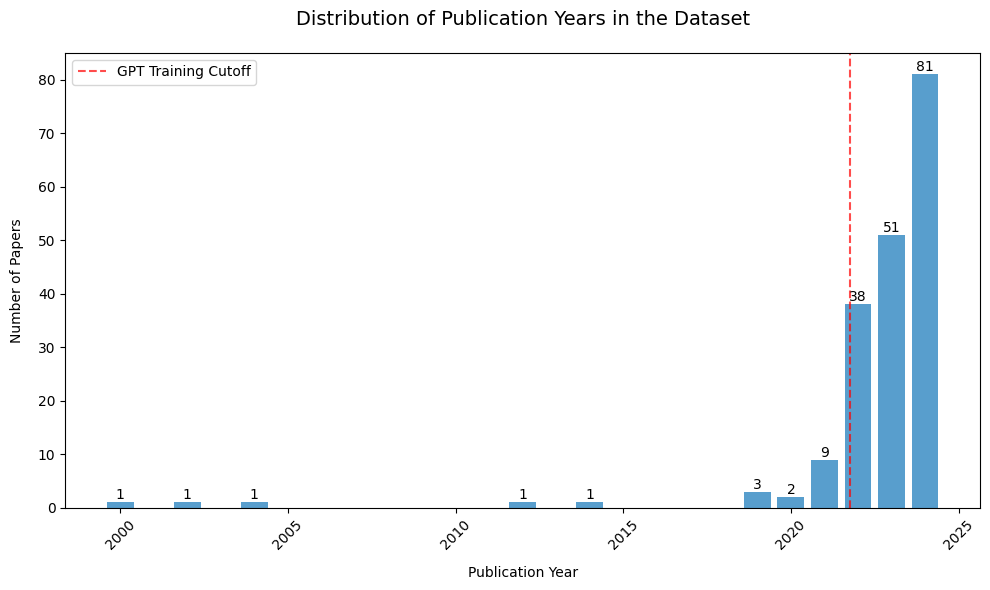
\includegraphics[width=\textwidth]{figures/paper_years.png}
    \caption{Distribution of the publication years of all of the papers in the LitQA dataset. The red line represents the training cutoff date for GPT.}
    \label{fig:paper-years}
\end{figure}

The data from HuggingFace, which contained the question, correct answer, and distractors, was loaded into a \texttt{pandas} DataFrame. For each question, the correct answer and distractors were shuffled and then assigned a letter to formulate a multiple-choice question.

\subsection{Result Reproduction}
After the dataset was finalized, the next step was to reproduce the original study's results using PaperQA.
The package provides an intuitive interface where the user calls the \texttt{ask} function (a synchronous wrapper for the asynchronous function \texttt{agent\_query}). This function uses the user's prompt to find relevant documents to answer the query. Each question was fed to the \texttt{agent\_query} function, and the resulting answer was recorded.

The standard output of PaperQA is a verbose summary that includes the answer, the reasoning behind the selection, and citations from the source papers. While this is a highly useful feature for researchers, its verbosity posed a challenge for the automated evaluation required by this project, which necessitated a single-letter answer for direct comparison against the ground truth. Initially, prompt engineering was employed to compel PaperQA to return only a single letter.\\

\begin{verbatim}
The following is a multiple choice question about biology.
Please answer by responding with the letter of the correct answer.

Think step by step.

{question}
\end{verbatim}

Where the question would contain the question and choices:

\begin{verbatim}
Question: Approximately what percentage of topologically associated 
domains in the GM12878 blood cell line does DiffDomain classify as 
reorganized in the K562 cell line? 
    A) 11%
    B) 41%
    C) 21%
    D) 51%
    E) 31%
    NA) Insufficient information to answer the question.
\end{verbatim}


Although this method produced a single-letter output, the agent invariably returned a short summary explaining its reasoning. 
This led to inconsistent outputs, where the position of the single-letter answer varied within the text, making it difficult to create a reliable evaluation pipeline. \\

The solution was to leverage structured outputs, which allow users to customize the exact output format of an LLM. However, PaperQA internally uses \texttt{LiteLLM} to invoke LLMs for tasks such as paper retrieval, evidence gathering, and answer generation. As structured output formats vary between different LLM providers and can typically only be used when calling models directly, there is no native entry point to enforce structured outputs within the PaperQA framework.

\subsection{Custom Multi-Agent Wrapper for PaperQA}
The solution to the structured output problem was to employ a multi-agent system, mirroring the architectural philosophy of PaperQA itself. Enforcing a JSON-style structured output was made possible by using a secondary agent system. 
Using a foundational `ConversableAgent`, a simple linear agentic system was developed to standardize the format of both the input to and the output from PaperQA. 
This ensured a consistent output format for evaluation. 
A diagram of this agent structure is required here.
The requirement for a standardized input format was driven by the specific needs of the evaluation methodology. 

\subsection{Evaluation and Inspect AI}

Inspect AI is a framework developed by the UK's AI Security Institute for evaluating the performance of LLMs. Its \texttt{eval} tool facilitates rapid performance evaluation by running LLM calls asynchronously. An \texttt{eval} task consists of three components: a dataset, a solver, and a scorer. The dataset is composed of \texttt{Sample} objects, each corresponding to an individual task (in this case, a multiple-choice question) and containing fields for the input, choices, and target answer. The solver represents the LLM system being evaluated, and the scorer defines the evaluation metric. A key benefit of Inspect AI is its provision of an intuitive interface for monitoring evaluation progress.\\

A separate custom library, \texttt{inspect\_evals}, exists for evaluating the performance of various LLMs on benchmarks such as LitQA \cite{laurent_lab-bench_2024}. However, it is only compatible with single LLMs, not multi-agent systems. \\

The \texttt{inspect\_ai} framework does offer support for multi-agent systems via its \texttt{bridge} function. However, the package is still in early development and, in its native form, does not support end-to-end evaluation of multi-agent systems on multiple-choice questions. The \texttt{bridge} function effectively allows a multi-agent system to act as the solver, but its communication format only supports the passing of agent messages, not structured data like the question, choices, or target answer. 
This limitation prevents the scorer from accessing the necessary information to determine if an answer is correct. \\

To overcome this, a custom package for multi-agent MCQ evaluation was developed using \texttt{inspect\_ai}. This package integrates with Inspect AI and allows any multi-agent system to be evaluated, provided it accepts a question and returns a text reply. 
It leverages a custom dataset builder that reads the \texttt{pandas} DataFrame and creates custom \texttt{Sample} objects with a structured JSON format. These samples are passed to a custom bridge agent that encapsulates the multi-agent system. The resulting answer is then evaluated by a custom scorer. Answers are classified as CORRECT, INCORRECT, or NA (for cases where the agent fails or cannot find an answer). This implementation was based on the logic in the \texttt{inspect\_evals} package. The custom scorer parses the structured output from the agent system and converts the data into an \texttt{inspect\_ai.Score} object, allowing the \texttt{eval} tool to calculate and aggregate performance metrics across the entire task. Below is an example prompt would be given into the \texttt{bridge} agent, which would partition the information and ensure the correct information is passed to the appropriate part of Inspect AI\\

\begin{figure}[H]
    \centering
    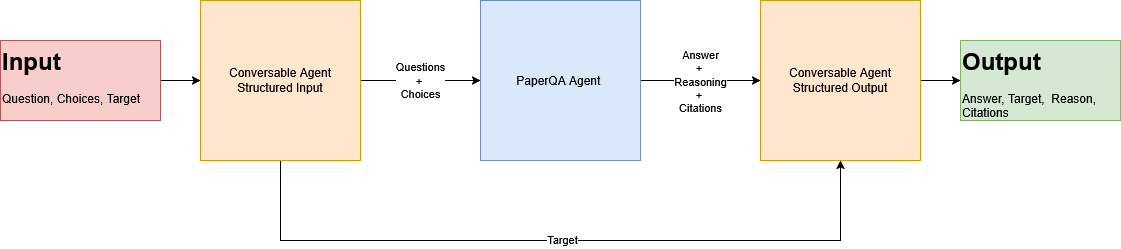
\includegraphics[width=\textwidth]{figures/bridge_agent.png}
    \caption{Custom Bridge Agent Structure}
    \label{fig:bridge_agent}
\end{figure}


\begin{verbatim}
Question: Approximately what percentage of topologically associated 
domains in the GM12878 blood cell line does DiffDomain classify as 
reorganized in the K562 cell line? 
    A) 11%
    B) 41%
    C) 21%
    D) 51%
    E) 31%
    NA) Insufficient information to answer the question.
    Target) E
\end{verbatim}



\subsection{Hyperparameters}

The main hyperparameter varied in this project was the LLM itself. In the original paper, GPT-4-Turbo was the default model. However, given the rapid pace of model development, several newer models were tested to assess performance improvements. The models evaluated were OpenAI's GPT-4o-Mini, GPT-4.1, and GPT-4-Turbo. Due to budget constraints, the default model used in our experiments was GPT-4o-Mini, which offers performance comparable to or better than GPT-4-Turbo for a lower per-token cost.\\

Another hyperparameter that was changed was the text embedding model. The default model used by PaperQA is OpenAI's \texttt{text-embedding-3-small}, which was no longer state-of-the-art at the time of the experiments. Instead, the highest-performing model available via LiteLLM, Google's \texttt{text-embedding-004}, was used. Embeddings are crucial for NLP tasks, as a more accurate semantic representation of text is hypothesized to improve an LLM's comprehension and subsequent decision-making. \\

Within PaperQA, there are also two key parameters that the original authors varied. First is the Answer Cutoff (\texttt{max\_sources}), which limits the maximum number of retrieved sources used to generate a response. This filtering occurs after the RCS step. The other hyperparameter is \texttt{evidence\_k} ('Consider Sources'), which controls the initial document retrieval step. To use an analogy: a researcher might retrieve the 30 most promising articles from a library (\texttt{evidence\_k} = 30). From these, they might skim the articles and select the best 5 (\texttt{max\_sources} = 5) to read thoroughly and inform their final answer. In the original paper, the default values for \texttt{max\_sources} and \texttt{evidence\_k} were 5 and 30, respectively. If \texttt{evidence\_k} is set lower than \texttt{max\_sources}, then \texttt{max\_sources} is automatically reduced to match. The authors also tested an \texttt{max\_sources} of 15 but found its performance to be worse; therefore, 5 was used as the default in our experiments.\\

PaperQA differentiates itself from other RAG systems by employing RCS. To test the criticality of this step, an experiment was also performed where RCS was disabled. \\

Other hyperparameters, such as temperature, were kept consistent throughout the experiments to make the results as reproducible as possible. \\


